\documentclass[12pt,a4paper]{article}

\usepackage[a4paper,text={16.5cm,25.2cm},centering]{geometry}
\usepackage{lmodern}
\usepackage{amssymb,amsmath}
\usepackage{caption}
\usepackage{subcaption}
\usepackage{bm}
\usepackage{graphicx}
\usepackage{microtype}
\usepackage{hyperref}
\usepackage{cleveref}
\usepackage{float}
\setlength{\parindent}{0pt}
\setlength{\parskip}{1.2ex}

% ---- All figures are not floating ---- %
% REMOVE WHEN NOT DRAFT
\makeatletter
\renewcommand*{\fps@figure}{H}
\renewcommand*{\fps@table}{H}
\makeatother
% -------------------------------------- %

\hypersetup
       {   pdfauthor = { Daniele Zago and Giovanna Capizzi },
           pdftitle={ Supplemental material },
           colorlinks=TRUE,
           linkcolor=black,
           citecolor=blue,
           urlcolor=blue
       }

\title{ Supplemental material }

\author{ Daniele Zago and Giovanna Capizzi }

\date{ 2022-09-28 }

\usepackage{upquote}
\usepackage{listings}
\usepackage{xcolor}
\lstset{
    basicstyle=\ttfamily\footnotesize,
    upquote=true,
    breaklines=true,
    breakindent=0pt,
    keepspaces=true,
    showspaces=false,
    columns=fullflexible,
    showtabs=false,
    showstringspaces=false,
    escapeinside={(*@}{@*)},
    extendedchars=true,
}
\newcommand{\HLJLt}[1]{#1}
\newcommand{\HLJLw}[1]{#1}
\newcommand{\HLJLe}[1]{#1}
\newcommand{\HLJLeB}[1]{#1}
\newcommand{\HLJLo}[1]{#1}
\newcommand{\HLJLk}[1]{\textcolor[RGB]{148,91,176}{\textbf{#1}}}
\newcommand{\HLJLkc}[1]{\textcolor[RGB]{59,151,46}{\textit{#1}}}
\newcommand{\HLJLkd}[1]{\textcolor[RGB]{214,102,97}{\textit{#1}}}
\newcommand{\HLJLkn}[1]{\textcolor[RGB]{148,91,176}{\textbf{#1}}}
\newcommand{\HLJLkp}[1]{\textcolor[RGB]{148,91,176}{\textbf{#1}}}
\newcommand{\HLJLkr}[1]{\textcolor[RGB]{148,91,176}{\textbf{#1}}}
\newcommand{\HLJLkt}[1]{\textcolor[RGB]{148,91,176}{\textbf{#1}}}
\newcommand{\HLJLn}[1]{#1}
\newcommand{\HLJLna}[1]{#1}
\newcommand{\HLJLnb}[1]{#1}
\newcommand{\HLJLnbp}[1]{#1}
\newcommand{\HLJLnc}[1]{#1}
\newcommand{\HLJLncB}[1]{#1}
\newcommand{\HLJLnd}[1]{\textcolor[RGB]{214,102,97}{#1}}
\newcommand{\HLJLne}[1]{#1}
\newcommand{\HLJLneB}[1]{#1}
\newcommand{\HLJLnf}[1]{\textcolor[RGB]{66,102,213}{#1}}
\newcommand{\HLJLnfm}[1]{\textcolor[RGB]{66,102,213}{#1}}
\newcommand{\HLJLnp}[1]{#1}
\newcommand{\HLJLnl}[1]{#1}
\newcommand{\HLJLnn}[1]{#1}
\newcommand{\HLJLno}[1]{#1}
\newcommand{\HLJLnt}[1]{#1}
\newcommand{\HLJLnv}[1]{#1}
\newcommand{\HLJLnvc}[1]{#1}
\newcommand{\HLJLnvg}[1]{#1}
\newcommand{\HLJLnvi}[1]{#1}
\newcommand{\HLJLnvm}[1]{#1}
\newcommand{\HLJLl}[1]{#1}
\newcommand{\HLJLld}[1]{\textcolor[RGB]{148,91,176}{\textit{#1}}}
\newcommand{\HLJLs}[1]{\textcolor[RGB]{201,61,57}{#1}}
\newcommand{\HLJLsa}[1]{\textcolor[RGB]{201,61,57}{#1}}
\newcommand{\HLJLsb}[1]{\textcolor[RGB]{201,61,57}{#1}}
\newcommand{\HLJLsc}[1]{\textcolor[RGB]{201,61,57}{#1}}
\newcommand{\HLJLsd}[1]{\textcolor[RGB]{201,61,57}{#1}}
\newcommand{\HLJLsdB}[1]{\textcolor[RGB]{201,61,57}{#1}}
\newcommand{\HLJLsdC}[1]{\textcolor[RGB]{201,61,57}{#1}}
\newcommand{\HLJLse}[1]{\textcolor[RGB]{59,151,46}{#1}}
\newcommand{\HLJLsh}[1]{\textcolor[RGB]{201,61,57}{#1}}
\newcommand{\HLJLsi}[1]{#1}
\newcommand{\HLJLso}[1]{\textcolor[RGB]{201,61,57}{#1}}
\newcommand{\HLJLsr}[1]{\textcolor[RGB]{201,61,57}{#1}}
\newcommand{\HLJLss}[1]{\textcolor[RGB]{201,61,57}{#1}}
\newcommand{\HLJLssB}[1]{\textcolor[RGB]{201,61,57}{#1}}
\newcommand{\HLJLnB}[1]{\textcolor[RGB]{59,151,46}{#1}}
\newcommand{\HLJLnbB}[1]{\textcolor[RGB]{59,151,46}{#1}}
\newcommand{\HLJLnfB}[1]{\textcolor[RGB]{59,151,46}{#1}}
\newcommand{\HLJLnh}[1]{\textcolor[RGB]{59,151,46}{#1}}
\newcommand{\HLJLni}[1]{\textcolor[RGB]{59,151,46}{#1}}
\newcommand{\HLJLnil}[1]{\textcolor[RGB]{59,151,46}{#1}}
\newcommand{\HLJLnoB}[1]{\textcolor[RGB]{59,151,46}{#1}}
\newcommand{\HLJLoB}[1]{\textcolor[RGB]{102,102,102}{\textbf{#1}}}
\newcommand{\HLJLow}[1]{\textcolor[RGB]{102,102,102}{\textbf{#1}}}
\newcommand{\HLJLp}[1]{#1}
\newcommand{\HLJLc}[1]{\textcolor[RGB]{153,153,119}{\textit{#1}}}
\newcommand{\HLJLch}[1]{\textcolor[RGB]{153,153,119}{\textit{#1}}}
\newcommand{\HLJLcm}[1]{\textcolor[RGB]{153,153,119}{\textit{#1}}}
\newcommand{\HLJLcp}[1]{\textcolor[RGB]{153,153,119}{\textit{#1}}}
\newcommand{\HLJLcpB}[1]{\textcolor[RGB]{153,153,119}{\textit{#1}}}
\newcommand{\HLJLcs}[1]{\textcolor[RGB]{153,153,119}{\textit{#1}}}
\newcommand{\HLJLcsB}[1]{\textcolor[RGB]{153,153,119}{\textit{#1}}}
\newcommand{\HLJLg}[1]{#1}
\newcommand{\HLJLgd}[1]{#1}
\newcommand{\HLJLge}[1]{#1}
\newcommand{\HLJLgeB}[1]{#1}
\newcommand{\HLJLgh}[1]{#1}
\newcommand{\HLJLgi}[1]{#1}
\newcommand{\HLJLgo}[1]{#1}
\newcommand{\HLJLgp}[1]{#1}
\newcommand{\HLJLgs}[1]{#1}
\newcommand{\HLJLgsB}[1]{#1}
\newcommand{\HLJLgt}[1]{#1}


\begin{document}

\maketitle

\section{In-depth analysis}
In this section we perform an in-depth analysis of the performance of the CLM and C&M2020 methods when changing the control chart design parameter.
Herein, the OC performance of the proposed cautious learning parameter update rules are compared to the fixed and adaptive estimators.
We use the same simulation settings as in Section ?? of the paper regarding the intial sample size, cautious learning parameters, parameter shift magnitude and location, and control limit design.
The IC process parameter is fixed to $\theta = 4$ and we study the performance of the proposed methodology as $ \lambda$ varies in $\{0.05, 0.075, 0.1, 0.125, 0.15, 0.175, 0.2\} $.
From the results in \Cref{fig:lambda=0.05/EWMA OC theta=4,fig:lambda=0.075/EWMA OC theta=4,fig:lambda=0.10/EWMA OC theta=4,fig:lambda=0.125/EWMA OC theta=4,fig:lambda=0.15/EWMA OC theta=4,fig:lambda=0.175/EWMA OC theta=4,fig:lambda=0.20/EWMA OC theta=4}, it is possible to see that the parameter estimator based on time-delayed update rules provide consistently improved results when compared to both adaptive and fixed estimators.
This appears to be valid across both shift sizes and control chart design parameter, with differences between the \textit{CLM and the C\&M2020 approaches}.
Overall, the suggested settings of $ A=1.5$ and $ B=50$ for the \textit{C\&M2020} update rule results in a more conservative update rule than the CLM approach.
Indeed, when the control chart displays a high sensitivity to small shifts such as in \Cref{fig:lambda=0.05/EWMA OC theta=4}, the CLM approach provides a protection against early shifts that is comparable to the \textit{C\&M2020} update rule.
However, the CLM approach provides a better protection to shifts that happen later in the monitoring phase due to the higher precision of the estimates.
Conversely, when the control chart is less sensitive to small parameter shifts (\Cref{fig:lambda=0.20/EWMA OC theta=4}), the conservativeness of the \textit{C\&M2020} approach is better apt at detecting early parameter shifts.
Overall, among the proposed delayed-parameter update rules we do not observe a clear winner, since the performance seems to depend on the sensitivity of the control chart to smaller or larger shifts.
Finally, the proposed delayed estimators appear to provide a better overall performance than the fully adaptive estimator, which shows degraded detection power when $ \tau=1$.

% --- Lambda = 0.05

% \begin{figure}
% \centering
% \begin{subfigure}{0.49\textwidth}
%   \centering
%   \caption{$ \delta = 0.25$}
%   \label{fig:lambda=0.05/theta=4.0/delta=0.25}
%   \includegraphics[width=\textwidth]{figures/sims/theta=4.0_signedEWMA(l = 0.05, upw = true, L = 1.0)/delta=0.25.png}
% \end{subfigure}
% \begin{subfigure}{0.49\textwidth}
%   \centering
%   \caption{$ \delta = 0.35$}
%   \label{fig:lambda=0.05/theta=4.0/delta=0.35}
%   \includegraphics[width=\textwidth]{figures/sims/theta=4.0_signedEWMA(l = 0.05, upw = true, L = 1.0)/delta=0.35.png}
% \end{subfigure}
% \begin{subfigure}{0.49\textwidth}
%   \centering
%   \caption{$ \delta = 0.5$}
%   \label{fig:lambda=0.05/theta=4.0/delta=0.5}
%   \includegraphics[width=\textwidth]{figures/sims/theta=4.0_signedEWMA(l = 0.05, upw = true, L = 1.0)/delta=0.50.png}
% \end{subfigure}
% \begin{subfigure}{0.49\textwidth}
%   \centering
%   \caption{$ \delta = 0.75$}
%   \label{fig:lambda=0.05/theta=4.0/delta=0.75}
%   \includegraphics[width=\textwidth]{figures/sims/theta=4.0_signedEWMA(l = 0.05, upw = true, L = 1.0)/delta=0.75.png}
% \end{subfigure}
% \begin{subfigure}{0.49\textwidth}
%   \centering
%   \caption{$ \delta = 1.0$}
%   \label{fig:lambda=0.05/theta=4.0/delta=1.0}
%   \includegraphics[width=\textwidth]{figures/sims/theta=4.0_signedEWMA(l = 0.05, upw = true, L = 1.0)/delta=1.00.png}
% \end{subfigure}
% \begin{subfigure}{0.49\textwidth}
%   \centering
%   \caption{$ \delta = 1.25$}
%   \label{fig:lambda=0.05/theta=4.0/delta=1.25}
%   \includegraphics[width=\textwidth]{figures/sims/theta=4.0_signedEWMA(l = 0.05, upw = true, L = 1.0)/delta=1.25.png}
% \end{subfigure}
%   \caption{OC performance of the EWMA ($ \lambda = 0.05$) control chart under fixed (FE), adaptive (AE), and cautious learning (CL) parameter updates when $ \gj = 4$.
%     Control charts satisfy the GICP condition \eqref{eq:GICP} with $ \beta = 0.1$.
%   Boxplots are based on the 200 simulated conditional ARLs.}
%   \label{fig:lambda=0.05/EWMA OC theta=4}
% \end{figure}

% \begin{figure}
%   \includegraphics[width=\textwidth]{figures/sims/theta=4.0_signedEWMA(l = 0.05, upw = true, L = 1.0)/OC-profiles.png}
%   \caption{Median of the OC conditional ARL of the EWMA-type control chart under fixed (FE), adaptive (AE), cautious learning (CL) parameter updates for $ \gj = 4$ and $ \lambda = 0.05$.
%     Control charts satisfy the GICP condition \eqref{eq:GICP} with $ \beta = 0.1$.
%   Plots are based on the 200 simulated conditional ARLs.}
%   \label{fig:lambda=0.05/EWMA OC profiles}
% \end{figure}

% --- Lambda = 0.075

% \begin{figure}
% \centering
% \begin{subfigure}{0.49\textwidth}
%   \centering
%   \caption{$ \delta = 0.25$}
%   \label{fig:lambda=0.075/theta=4.0/delta=0.25}
%   \includegraphics[width=\textwidth]{figures/sims/theta=4.0_signedEWMA(l = 0.075, upw = true, L = 1.0)/delta=0.25.png}
% \end{subfigure}
% \begin{subfigure}{0.49\textwidth}
%   \centering
%   \caption{$ \delta = 0.35$}
%   \label{fig:lambda=0.075/theta=4.0/delta=0.35}
%   \includegraphics[width=\textwidth]{figures/sims/theta=4.0_signedEWMA(l = 0.075, upw = true, L = 1.0)/delta=0.35.png}
% \end{subfigure}
% \begin{subfigure}{0.49\textwidth}
%   \centering
%   \caption{$ \delta = 0.5$}
%   \label{fig:lambda=0.075/theta=4.0/delta=0.5}
%   \includegraphics[width=\textwidth]{figures/sims/theta=4.0_signedEWMA(l = 0.075, upw = true, L = 1.0)/delta=0.50.png}
% \end{subfigure}
% \begin{subfigure}{0.49\textwidth}
%   \centering
%   \caption{$ \delta = 0.75$}
%   \label{fig:lambda=0.075/theta=4.0/delta=0.75}
%   \includegraphics[width=\textwidth]{figures/sims/theta=4.0_signedEWMA(l = 0.075, upw = true, L = 1.0)/delta=0.75.png}
% \end{subfigure}
% \begin{subfigure}{0.49\textwidth}
%   \centering
%   \caption{$ \delta = 1.0$}
%   \label{fig:lambda=0.075/theta=4.0/delta=1.0}
%   \includegraphics[width=\textwidth]{figures/sims/theta=4.0_signedEWMA(l = 0.075, upw = true, L = 1.0)/delta=1.00.png}
% \end{subfigure}
% \begin{subfigure}{0.49\textwidth}
%   \centering
%   \caption{$ \delta = 1.25$}
%   \label{fig:lambda=0.075/theta=4.0/delta=1.25}
%   \includegraphics[width=\textwidth]{figures/sims/theta=4.0_signedEWMA(l = 0.075, upw = true, L = 1.0)/delta=1.25.png}
% \end{subfigure}
%   \caption{OC performance of the EWMA ($ \lambda = 0.075$) control chart under fixed (FE), adaptive (AE), and cautious learning (CL) parameter updates when $ \gj = 4$.
%     Control charts satisfy the GICP condition \eqref{eq:GICP} with $ \beta = 0.1$.
%   Boxplots are based on the 200 simulated conditional ARLs.}
%   \label{fig:lambda=0.075/EWMA OC theta=4}
% \end{figure}

% \begin{figure}
%   \includegraphics[width=\textwidth]{figures/sims/theta=4.0_signedEWMA(l = 0.075, upw = true, L = 1.0)/OC-profiles.png}
%   \caption{Median of the OC conditional ARL of the EWMA-type control chart under fixed (FE), adaptive (AE), cautious learning (CL) parameter updates for $ \gj = 4$ and $ \lambda = 0.075$.
%     Control charts satisfy the GICP condition \eqref{eq:GICP} with $ \beta = 0.1$.
%   Plots are based on the 200 simulated conditional ARLs.}
%   \label{fig:lambda=0.05/EWMA OC profiles}
% \end{figure}

% --- Lambda = 0.1

% \begin{figure}
% \centering
% \begin{subfigure}{0.49\textwidth}
%   \centering
%   \caption{$ \delta = 0.25$}
%   \label{fig:lambda=0.10/theta=4.0/delta=0.25}
%   \includegraphics[width=\textwidth]{figures/sims/theta=4.0_signedEWMA(l = 0.1, upw = true, L = 1.0)/delta=0.25.png}
% \end{subfigure}
% \begin{subfigure}{0.49\textwidth}
%   \centering
%   \caption{$ \delta = 0.35$}
%   \label{fig:lambda=0.10/theta=4.0/delta=0.35}
%   \includegraphics[width=\textwidth]{figures/sims/theta=4.0_signedEWMA(l = 0.1, upw = true, L = 1.0)/delta=0.35.png}
% \end{subfigure}
% \begin{subfigure}{0.49\textwidth}
%   \centering
%   \caption{$ \delta = 0.5$}
%   \label{fig:lambda=0.10/theta=4.0/delta=0.5}
%   \includegraphics[width=\textwidth]{figures/sims/theta=4.0_signedEWMA(l = 0.1, upw = true, L = 1.0)/delta=0.50.png}
% \end{subfigure}
% \begin{subfigure}{0.49\textwidth}
%   \centering
%   \caption{$ \delta = 0.75$}
%   \label{fig:lambda=0.10/theta=4.0/delta=0.75}
%   \includegraphics[width=\textwidth]{figures/sims/theta=4.0_signedEWMA(l = 0.1, upw = true, L = 1.0)/delta=0.75.png}
% \end{subfigure}
% \begin{subfigure}{0.49\textwidth}
%   \centering
%   \caption{$ \delta = 1.0$}
%   \label{fig:lambda=0.10/theta=4.0/delta=1.0}
%   \includegraphics[width=\textwidth]{figures/sims/theta=4.0_signedEWMA(l = 0.1, upw = true, L = 1.0)/delta=1.00.png}
% \end{subfigure}
% \begin{subfigure}{0.49\textwidth}
%   \centering
%   \caption{$ \delta = 1.25$}
%   \label{fig:lambda=0.10/theta=4.0/delta=1.25}
%   \includegraphics[width=\textwidth]{figures/sims/theta=4.0_signedEWMA(l = 0.1, upw = true, L = 1.0)/delta=1.25.png}
% \end{subfigure}
%   \caption{OC performance of the EWMA ($ \lambda = 0.1$) control chart under fixed (FE), adaptive (AE), and cautious learning (CL) parameter updates when $ \gj = 4$.
%     Control charts satisfy the GICP condition \eqref{eq:GICP} with $ \beta = 0.1$.
%   Boxplots are based on the 200 simulated conditional ARLs.}
%   \label{fig:lambda=0.10/EWMA OC theta=4}
% \end{figure}

% \begin{figure}
%   \includegraphics[width=\textwidth]{figures/sims/theta=4.0_signedEWMA(l = 0.1, upw = true, L = 1.0)/OC-profiles.png}
%   \caption{Median of the OC conditional ARL of the EWMA-type control chart under fixed (FE), adaptive (AE), cautious learning (CL) parameter updates for $ \gj = 4$ and $ \lambda = 0.1$.
%     Control charts satisfy the GICP condition \eqref{eq:GICP} with $ \beta = 0.1$.
%   Plots are based on the 200 simulated conditional ARLs.}
%   \label{fig:lambda=0.05/EWMA OC profiles}
% \end{figure}

% --- Lambda = 0.125

% \begin{figure}
% \centering
% \begin{subfigure}{0.49\textwidth}
%   \centering
%   \caption{$ \delta = 0.25$}
%   \label{fig:lambda=0.125/theta=4.0/delta=0.25}
%   \includegraphics[width=\textwidth]{figures/sims/theta=4.0_signedEWMA(l = 0.125, upw = true, L = 1.0)/delta=0.25.png}
% \end{subfigure}
% \begin{subfigure}{0.49\textwidth}
%   \centering
%   \caption{$ \delta = 0.35$}
%   \label{fig:lambda=0.125/theta=4.0/delta=0.35}
%   \includegraphics[width=\textwidth]{figures/sims/theta=4.0_signedEWMA(l = 0.125, upw = true, L = 1.0)/delta=0.35.png}
% \end{subfigure}
% \begin{subfigure}{0.49\textwidth}
%   \centering
%   \caption{$ \delta = 0.5$}
%   \label{fig:lambda=0.125/theta=4.0/delta=0.5}
%   \includegraphics[width=\textwidth]{figures/sims/theta=4.0_signedEWMA(l = 0.125, upw = true, L = 1.0)/delta=0.50.png}
% \end{subfigure}
% \begin{subfigure}{0.49\textwidth}
%   \centering
%   \caption{$ \delta = 0.75$}
%   \label{fig:lambda=0.125/theta=4.0/delta=0.75}
%   \includegraphics[width=\textwidth]{figures/sims/theta=4.0_signedEWMA(l = 0.125, upw = true, L = 1.0)/delta=0.75.png}
% \end{subfigure}
% \begin{subfigure}{0.49\textwidth}
%   \centering
%   \caption{$ \delta = 1.0$}
%   \label{fig:lambda=0.125/theta=4.0/delta=1.0}
%   \includegraphics[width=\textwidth]{figures/sims/theta=4.0_signedEWMA(l = 0.125, upw = true, L = 1.0)/delta=1.00.png}
% \end{subfigure}
% \begin{subfigure}{0.49\textwidth}
%   \centering
%   \caption{$ \delta = 1.25$}
%   \label{fig:lambda=0.125/theta=4.0/delta=1.25}
%   \includegraphics[width=\textwidth]{figures/sims/theta=4.0_signedEWMA(l = 0.125, upw = true, L = 1.0)/delta=1.25.png}
% \end{subfigure}
%   \caption{OC performance of the EWMA ($ \lambda = 0.125$) control chart under fixed (FE), adaptive (AE), and cautious learning (CL) parameter updates when $ \gj = 4$.
%     Control charts satisfy the GICP condition \eqref{eq:GICP} with $ \beta = 0.1$.
%   Boxplots are based on the 200 simulated conditional ARLs.}
%   \label{fig:lambda=0.125/EWMA OC theta=4}
% \end{figure}

% \begin{figure}
%   \includegraphics[width=\textwidth]{figures/sims/theta=4.0_signedEWMA(l = 0.125, upw = true, L = 1.0)/OC-profiles.png}
%   \caption{Median of the OC conditional ARL of the EWMA-type control chart under fixed (FE), adaptive (AE), cautious learning (CL) parameter updates for $ \gj = 4$ and $ \lambda = 0.125$.
%     Control charts satisfy the GICP condition \eqref{eq:GICP} with $ \beta = 0.1$.
%   Plots are based on the 200 simulated conditional ARLs.}
%   \label{fig:lambda=0.05/EWMA OC profiles}
% \end{figure}

% --- Lambda = 0.15

% \begin{figure}
% \centering
% \begin{subfigure}{0.49\textwidth}
%   \centering
%   \caption{$ \delta = 0.25$}
%   \label{fig:lambda=0.15/theta=4.0/delta=0.25}
%   \includegraphics[width=\textwidth]{figures/sims/theta=4.0_signedEWMA(l = 0.15, upw = true, L = 1.0)/delta=0.25.png}
% \end{subfigure}
% \begin{subfigure}{0.49\textwidth}
%   \centering
%   \caption{$ \delta = 0.35$}
%   \label{fig:lambda=0.15/theta=4.0/delta=0.35}
%   \includegraphics[width=\textwidth]{figures/sims/theta=4.0_signedEWMA(l = 0.15, upw = true, L = 1.0)/delta=0.35.png}
% \end{subfigure}
% \begin{subfigure}{0.49\textwidth}
%   \centering
%   \caption{$ \delta = 0.5$}
%   \label{fig:lambda=0.15/theta=4.0/delta=0.5}
%   \includegraphics[width=\textwidth]{figures/sims/theta=4.0_signedEWMA(l = 0.15, upw = true, L = 1.0)/delta=0.50.png}
% \end{subfigure}
% \begin{subfigure}{0.49\textwidth}
%   \centering
%   \caption{$ \delta = 0.75$}
%   \label{fig:lambda=0.15/theta=4.0/delta=0.75}
%   \includegraphics[width=\textwidth]{figures/sims/theta=4.0_signedEWMA(l = 0.15, upw = true, L = 1.0)/delta=0.75.png}
% \end{subfigure}
% \begin{subfigure}{0.49\textwidth}
%   \centering
%   \caption{$ \delta = 1.0$}
%   \label{fig:lambda=0.15/theta=4.0/delta=1.0}
%   \includegraphics[width=\textwidth]{figures/sims/theta=4.0_signedEWMA(l = 0.15, upw = true, L = 1.0)/delta=1.00.png}
% \end{subfigure}
% \begin{subfigure}{0.49\textwidth}
%   \centering
%   \caption{$ \delta = 1.25$}
%   \label{fig:lambda=0.15/theta=4.0/delta=1.25}
%   \includegraphics[width=\textwidth]{figures/sims/theta=4.0_signedEWMA(l = 0.15, upw = true, L = 1.0)/delta=1.25.png}
% \end{subfigure}
%   \caption{OC performance of the EWMA ($ \lambda = 0.15$) control chart under fixed (FE), adaptive (AE), and cautious learning (CL) parameter updates when $ \gj = 4$.
%     Control charts satisfy the GICP condition \eqref{eq:GICP} with $ \beta = 0.1$.
%   Boxplots are based on the 200 simulated conditional ARLs.}
%   \label{fig:lambda=0.15/EWMA OC theta=4}
% \end{figure}

% \begin{figure}
%   \includegraphics[width=\textwidth]{figures/sims/theta=4.0_signedEWMA(l = 0.15, upw = true, L = 1.0)/OC-profiles.png}
%   \caption{Median of the OC conditional ARL of the EWMA-type control chart under fixed (FE), adaptive (AE), cautious learning (CL) parameter updates for $ \gj = 4$ and $ \lambda = 0.15$.
%     Control charts satisfy the GICP condition \eqref{eq:GICP} with $ \beta = 0.1$.
%   Plots are based on the 200 simulated conditional ARLs.}
%   \label{fig:lambda=0.05/EWMA OC profiles}
% \end{figure}

% --- Lambda = 0.175

% \begin{figure}
% \centering
% \begin{subfigure}{0.49\textwidth}
%   \centering
%   \caption{$ \delta = 0.25$}
%   \label{fig:lambda=0.175/theta=4.0/delta=0.25}
%   \includegraphics[width=\textwidth]{figures/sims/theta=4.0_signedEWMA(l = 0.175, upw = true, L = 1.0)/delta=0.25.png}
% \end{subfigure}
% \begin{subfigure}{0.49\textwidth}
%   \centering
%   \caption{$ \delta = 0.35$}
%   \label{fig:lambda=0.175/theta=4.0/delta=0.35}
%   \includegraphics[width=\textwidth]{figures/sims/theta=4.0_signedEWMA(l = 0.175, upw = true, L = 1.0)/delta=0.35.png}
% \end{subfigure}
% \begin{subfigure}{0.49\textwidth}
%   \centering
%   \caption{$ \delta = 0.5$}
%   \label{fig:lambda=0.175/theta=4.0/delta=0.5}
%   \includegraphics[width=\textwidth]{figures/sims/theta=4.0_signedEWMA(l = 0.175, upw = true, L = 1.0)/delta=0.50.png}
% \end{subfigure}
% \begin{subfigure}{0.49\textwidth}
%   \centering
%   \caption{$ \delta = 0.75$}
%   \label{fig:lambda=0.175/theta=4.0/delta=0.75}
%   \includegraphics[width=\textwidth]{figures/sims/theta=4.0_signedEWMA(l = 0.175, upw = true, L = 1.0)/delta=0.75.png}
% \end{subfigure}
% \begin{subfigure}{0.49\textwidth}
%   \centering
%   \caption{$ \delta = 1.0$}
%   \label{fig:lambda=0.175/theta=4.0/delta=1.0}
%   \includegraphics[width=\textwidth]{figures/sims/theta=4.0_signedEWMA(l = 0.175, upw = true, L = 1.0)/delta=1.00.png}
% \end{subfigure}
% \begin{subfigure}{0.49\textwidth}
%   \centering
%   \caption{$ \delta = 1.25$}
%   \label{fig:lambda=0.175/theta=4.0/delta=1.25}
%   \includegraphics[width=\textwidth]{figures/sims/theta=4.0_signedEWMA(l = 0.175, upw = true, L = 1.0)/delta=1.25.png}
% \end{subfigure}
%   \caption{OC performance of the EWMA ($ \lambda = 0.175$) control chart under fixed (FE), adaptive (AE), and cautious learning (CL) parameter updates when $ \gj = 4$.
%     Control charts satisfy the GICP condition \eqref{eq:GICP} with $ \beta = 0.1$.
%   Boxplots are based on the 200 simulated conditional ARLs.}
%   \label{fig:lambda=0.175/EWMA OC theta=4}
% \end{figure}

% \begin{figure}
%   \includegraphics[width=\textwidth]{figures/sims/theta=4.0_signedEWMA(l = 0.175, upw = true, L = 1.0)/OC-profiles.png}
%   \caption{Median of the OC conditional ARL of the EWMA-type control chart under fixed (FE), adaptive (AE), cautious learning (CL) parameter updates for $ \gj = 4$ and $ \lambda = 0.175$.
%     Control charts satisfy the GICP condition \eqref{eq:GICP} with $ \beta = 0.1$.
%   Plots are based on the 200 simulated conditional ARLs.}
%   \label{fig:lambda=0.05/EWMA OC profiles}
% \end{figure}

% --- Lambda = 0.2

% \begin{figure}
% \centering
% \begin{subfigure}{0.49\textwidth}
%   \centering
%   \caption{$ \delta = 0.25$}
%   \label{fig:lambda=0.20/theta=4.0/delta=0.25}
%   \includegraphics[width=\textwidth]{figures/sims/theta=4.0_signedEWMA(l = 0.2, upw = true, L = 1.0)/delta=0.25.png}
% \end{subfigure}
% \begin{subfigure}{0.49\textwidth}
%   \centering
%   \caption{$ \delta = 0.35$}
%   \label{fig:lambda=0.20/theta=4.0/delta=0.35}
%   \includegraphics[width=\textwidth]{figures/sims/theta=4.0_signedEWMA(l = 0.2, upw = true, L = 1.0)/delta=0.35.png}
% \end{subfigure}
% \begin{subfigure}{0.49\textwidth}
%   \centering
%   \caption{$ \delta = 0.5$}
%   \label{fig:lambda=0.20/theta=4.0/delta=0.5}
%   \includegraphics[width=\textwidth]{figures/sims/theta=4.0_signedEWMA(l = 0.2, upw = true, L = 1.0)/delta=0.50.png}
% \end{subfigure}
% \begin{subfigure}{0.49\textwidth}
%   \centering
%   \caption{$ \delta = 0.75$}
%   \label{fig:lambda=0.20/theta=4.0/delta=0.75}
%   \includegraphics[width=\textwidth]{figures/sims/theta=4.0_signedEWMA(l = 0.2, upw = true, L = 1.0)/delta=0.75.png}
% \end{subfigure}
% \begin{subfigure}{0.49\textwidth}
%   \centering
%   \caption{$ \delta = 1.0$}
%   \label{fig:lambda=0.20/theta=4.0/delta=1.0}
%   \includegraphics[width=\textwidth]{figures/sims/theta=4.0_signedEWMA(l = 0.2, upw = true, L = 1.0)/delta=1.00.png}
% \end{subfigure}
% \begin{subfigure}{0.49\textwidth}
%   \centering
%   \caption{$ \delta = 1.25$}
%   \label{fig:lambda=0.20/theta=4.0/delta=1.25}
%   \includegraphics[width=\textwidth]{figures/sims/theta=4.0_signedEWMA(l = 0.2, upw = true, L = 1.0)/delta=1.25.png}
% \end{subfigure}
%   \caption{OC performance of the EWMA ($ \lambda = 0.2$) control chart under fixed (FE), adaptive (AE), and cautious learning (CL) parameter updates when $ \gj = 4$.
%     Control charts satisfy the GICP condition \eqref{eq:GICP} with $ \beta = 0.1$.
%   Boxplots are based on the 200 simulated conditional ARLs.}
%   \label{fig:lambda=0.20/EWMA OC theta=4}
% \end{figure}

% \begin{figure}
%   \includegraphics[width=\textwidth]{figures/sims/theta=4.0_signedEWMA(l = 0.2, upw = true, L = 1.0)/OC-profiles.png}
%   \caption{Median of the OC conditional ARL of the EWMA-type control chart under fixed (FE), adaptive (AE), cautious learning (CL) parameter updates for $ \gj = 4$ and $ \lambda = 0.2$.
%     Control charts satisfy the GICP condition \eqref{eq:GICP} with $ \beta = 0.1$.
%   Plots are based on the 200 simulated conditional ARLs.}
%   \label{fig:lambda=0.20/EWMA OC profiles}
% \end{figure}


\section{Application to the ICU admissions data}
Here, we implement the code that reproduces the analysis on the ICU dataset in Section 5 of the paper.

First, we load the necessary packages and the environment variables that are provided in the source code.



\begin{lstlisting}
(*@\HLJLk{using}@*) (*@\HLJLn{DrWatson}@*)
(*@\HLJLcs{{\#}@quickactivate}@*) (*@\HLJLcs{"{}CautiousLearning"{}}@*)
(*@\HLJLnf{quickactivate}@*)(*@\HLJLp{(}@*)(*@\HLJLs{"{}}@*)(*@\HLJLsi{{\$}}@*)(*@\HLJLp{(}@*)(*@\HLJLnf{homedir}@*)(*@\HLJLp{())}@*)(*@\HLJLs{/Documents/git/SPC/CautiousLearning"{}}@*)(*@\HLJLp{)}@*)

(*@\HLJLk{using}@*) (*@\HLJLn{Distributions}@*)(*@\HLJLp{,}@*) (*@\HLJLn{Random}@*)
(*@\HLJLk{using}@*) (*@\HLJLn{Parameters}@*)
(*@\HLJLk{using}@*) (*@\HLJLn{SharedArrays}@*)
(*@\HLJLk{using}@*) (*@\HLJLn{DataFrames}@*)(*@\HLJLp{,}@*) (*@\HLJLn{CSV}@*)(*@\HLJLp{,}@*) (*@\HLJLn{Dates}@*)
(*@\HLJLk{using}@*) (*@\HLJLn{Plots}@*)(*@\HLJLp{,}@*) (*@\HLJLn{StatsBase}@*)(*@\HLJLp{,}@*) (*@\HLJLn{StatsPlots}@*)(*@\HLJLp{,}@*) (*@\HLJLn{LaTeXStrings}@*)(*@\HLJLp{,}@*) (*@\HLJLn{RCall}@*)
(*@\HLJLk{using}@*) (*@\HLJLn{StatisticalProcessControl}@*)

(*@\HLJLnf{include}@*)(*@\HLJLp{(}@*)(*@\HLJLnf{srcdir}@*)(*@\HLJLp{(}@*)(*@\HLJLs{"{}generate{\_}data.jl"{}}@*)(*@\HLJLp{))}@*)
(*@\HLJLnf{include}@*)(*@\HLJLp{(}@*)(*@\HLJLnf{srcdir}@*)(*@\HLJLp{(}@*)(*@\HLJLs{"{}update{\_}parameter.jl"{}}@*)(*@\HLJLp{))}@*)
(*@\HLJLnf{include}@*)(*@\HLJLp{(}@*)(*@\HLJLnf{srcdir}@*)(*@\HLJLp{(}@*)(*@\HLJLs{"{}simulate{\_}runs.jl"{}}@*)(*@\HLJLp{))}@*)
(*@\HLJLnf{include}@*)(*@\HLJLp{(}@*)(*@\HLJLnf{srcdir}@*)(*@\HLJLp{(}@*)(*@\HLJLs{"{}cfg.jl"{}}@*)(*@\HLJLp{))}@*)
\end{lstlisting}


First, we load the dataset which is located in the \texttt{data/ICUadmissions} folder, relative to the main directory of the project. We consider the data concerning the New York City area in 2020.


\begin{lstlisting}
(*@\HLJLn{fold}@*) (*@\HLJLoB{=}@*) (*@\HLJLs{"{}ICUadmissions"{}}@*)
(*@\HLJLn{dat}@*) (*@\HLJLoB{=}@*) (*@\HLJLnf{DataFrame}@*)(*@\HLJLp{(}@*)(*@\HLJLn{CSV}@*)(*@\HLJLoB{.}@*)(*@\HLJLnf{File}@*)(*@\HLJLp{(}@*)(*@\HLJLnf{datadir}@*)(*@\HLJLp{(}@*)(*@\HLJLn{fold}@*)(*@\HLJLp{,}@*) (*@\HLJLs{"{}New{\_}York{\_}Forward{\_}COVID-19{\_}Daily{\_}Hospitalization{\_}Summary{\_}by{\_}Region.csv"{}}@*)(*@\HLJLp{)))}@*)
(*@\HLJLn{nydat}@*) (*@\HLJLoB{=}@*) (*@\HLJLnf{filter}@*)(*@\HLJLp{(}@*)(*@\HLJLn{row}@*) (*@\HLJLoB{->}@*) (*@\HLJLn{row}@*)(*@\HLJLoB{.}@*)(*@\HLJLn{Region}@*) (*@\HLJLoB{==}@*) (*@\HLJLs{"{}NEW}@*) (*@\HLJLs{YORK}@*) (*@\HLJLs{CITY"{}}@*)(*@\HLJLp{,}@*) (*@\HLJLn{dat}@*)(*@\HLJLp{)}@*)
(*@\HLJLn{nydat}@*)(*@\HLJLoB{.}@*)(*@\HLJLn{date}@*) (*@\HLJLoB{.=}@*) (*@\HLJLn{Date}@*)(*@\HLJLoB{.}@*)(*@\HLJLp{(}@*)(*@\HLJLn{nydat}@*)(*@\HLJLp{[}@*)(*@\HLJLoB{:}@*)(*@\HLJLp{,}@*) (*@\HLJLni{1}@*)(*@\HLJLp{],}@*) (*@\HLJLso{dateformat"{}mm/dd/yyyy"{}}@*)(*@\HLJLp{)}@*)
(*@\HLJLn{nydat}@*) (*@\HLJLoB{=}@*) (*@\HLJLnf{filter}@*)(*@\HLJLp{(}@*)(*@\HLJLn{row}@*) (*@\HLJLoB{->}@*) (*@\HLJLnf{year}@*)(*@\HLJLp{(}@*)(*@\HLJLn{row}@*)(*@\HLJLoB{.}@*)(*@\HLJLn{date}@*)(*@\HLJLp{)}@*) (*@\HLJLoB{==}@*) (*@\HLJLni{2020}@*)(*@\HLJLp{,}@*) (*@\HLJLn{nydat}@*)(*@\HLJLp{);}@*)
\end{lstlisting}


We obtain the daily ICU counts along with the corresponding dates, which start from March 2020.


\begin{lstlisting}
(*@\HLJLk{using}@*) (*@\HLJLn{Plots}@*)(*@\HLJLoB{.}@*)(*@\HLJLn{PlotMeasures}@*)
(*@\HLJLn{y2020}@*) (*@\HLJLoB{=}@*) (*@\HLJLn{nydat}@*)(*@\HLJLp{[}@*)(*@\HLJLoB{:}@*)(*@\HLJLp{,}@*) (*@\HLJLni{4}@*)(*@\HLJLp{]}@*)
(*@\HLJLn{days2020}@*) (*@\HLJLoB{=}@*) (*@\HLJLn{nydat}@*)(*@\HLJLp{[}@*)(*@\HLJLoB{:}@*)(*@\HLJLp{,}@*) (*@\HLJLni{5}@*)(*@\HLJLp{]}@*)
(*@\HLJLnf{first}@*)(*@\HLJLp{(}@*)(*@\HLJLn{y2020}@*)(*@\HLJLp{,}@*) (*@\HLJLni{10}@*)(*@\HLJLp{)}@*)
(*@\HLJLnf{first}@*)(*@\HLJLp{(}@*)(*@\HLJLn{days2020}@*)(*@\HLJLp{,}@*) (*@\HLJLni{10}@*)(*@\HLJLp{)}@*)
\end{lstlisting}

\begin{lstlisting}
10-element Vector(*@{{\{}}@*)Dates.Date(*@{{\}}}@*):
 2020-03-26
 2020-03-27
 2020-03-28
 2020-03-29
 2020-03-30
 2020-03-31
 2020-04-01
 2020-04-02
 2020-04-03
 2020-04-04
\end{lstlisting}


Then, we select the indices of the IC/OC datasets along with the initial sample size and prospective monitoring size. The following code reproduces Figure ?? in the paper.


\begin{lstlisting}
(*@\HLJLcs{{\#}}@*) (*@\HLJLcs{ic{\_}2020}@*) (*@\HLJLcs{=}@*) (*@\HLJLcs{115:175}@*)
(*@\HLJLn{ic{\_}2020}@*) (*@\HLJLoB{=}@*) (*@\HLJLni{115}@*)(*@\HLJLoB{:}@*)(*@\HLJLni{155}@*)
(*@\HLJLn{oc{\_}2020}@*) (*@\HLJLoB{=}@*) (*@\HLJLp{(}@*)(*@\HLJLn{ic{\_}2020}@*)(*@\HLJLp{[}@*)(*@\HLJLk{end}@*)(*@\HLJLp{]}@*)(*@\HLJLoB{+}@*)(*@\HLJLni{1}@*)(*@\HLJLp{)}@*)(*@\HLJLoB{:}@*)(*@\HLJLnf{length}@*)(*@\HLJLp{(}@*)(*@\HLJLn{y2020}@*)(*@\HLJLp{)}@*)
(*@\HLJLn{n{\_}ic}@*) (*@\HLJLoB{=}@*) (*@\HLJLnf{length}@*)(*@\HLJLp{(}@*)(*@\HLJLn{ic{\_}2020}@*)(*@\HLJLp{)}@*)
(*@\HLJLn{n{\_}oc}@*) (*@\HLJLoB{=}@*) (*@\HLJLnf{length}@*)(*@\HLJLp{(}@*)(*@\HLJLn{oc{\_}2020}@*)(*@\HLJLp{)}@*)
(*@\HLJLn{pl}@*) (*@\HLJLoB{=}@*) (*@\HLJLnf{plot}@*)(*@\HLJLp{(}@*)(*@\HLJLn{days2020}@*)(*@\HLJLp{,}@*) (*@\HLJLn{y2020}@*)(*@\HLJLp{,}@*) (*@\HLJLn{label}@*)(*@\HLJLoB{=}@*)(*@\HLJLs{"{}"{}}@*)(*@\HLJLp{,}@*) (*@\HLJLn{dpi}@*)(*@\HLJLoB{=}@*)(*@\HLJLni{400}@*)(*@\HLJLp{,}@*) (*@\HLJLn{xrotation}@*)(*@\HLJLoB{=}@*)(*@\HLJLni{45}@*)(*@\HLJLp{,}@*) (*@\HLJLn{bottom{\_}margin}@*)(*@\HLJLoB{=}@*)(*@\HLJLni{3}@*)(*@\HLJLn{mm}@*)(*@\HLJLp{)}@*)
(*@\HLJLnf{plot!}@*)(*@\HLJLp{(}@*)(*@\HLJLn{pl}@*)(*@\HLJLp{,}@*) (*@\HLJLn{days2020}@*)(*@\HLJLp{[}@*)(*@\HLJLn{ic{\_}2020}@*)(*@\HLJLp{],}@*) (*@\HLJLnf{fill}@*)(*@\HLJLp{(}@*)(*@\HLJLni{0}@*)(*@\HLJLp{,}@*) (*@\HLJLn{n{\_}ic}@*)(*@\HLJLp{),}@*) (*@\HLJLn{fillrange}@*)(*@\HLJLoB{=}@*)(*@\HLJLnf{fill}@*)(*@\HLJLp{(}@*)(*@\HLJLnf{maximum}@*)(*@\HLJLp{(}@*)(*@\HLJLn{y2020}@*)(*@\HLJLp{),}@*) (*@\HLJLn{n{\_}ic}@*)(*@\HLJLp{),}@*) (*@\HLJLn{color}@*)(*@\HLJLoB{=:}@*)(*@\HLJLn{gray}@*)(*@\HLJLp{,}@*) (*@\HLJLn{fillcolor}@*) (*@\HLJLoB{=}@*) (*@\HLJLs{"{}gray"{}}@*)(*@\HLJLp{,}@*) (*@\HLJLn{fillalpha}@*)(*@\HLJLoB{=}@*)(*@\HLJLnfB{0.25}@*)(*@\HLJLp{,}@*) (*@\HLJLn{alpha}@*)(*@\HLJLoB{=}@*)(*@\HLJLnfB{0.0}@*)(*@\HLJLp{,}@*) (*@\HLJLn{label}@*)(*@\HLJLoB{=}@*)(*@\HLJLs{"{}IC"{}}@*)(*@\HLJLp{)}@*)
\end{lstlisting}

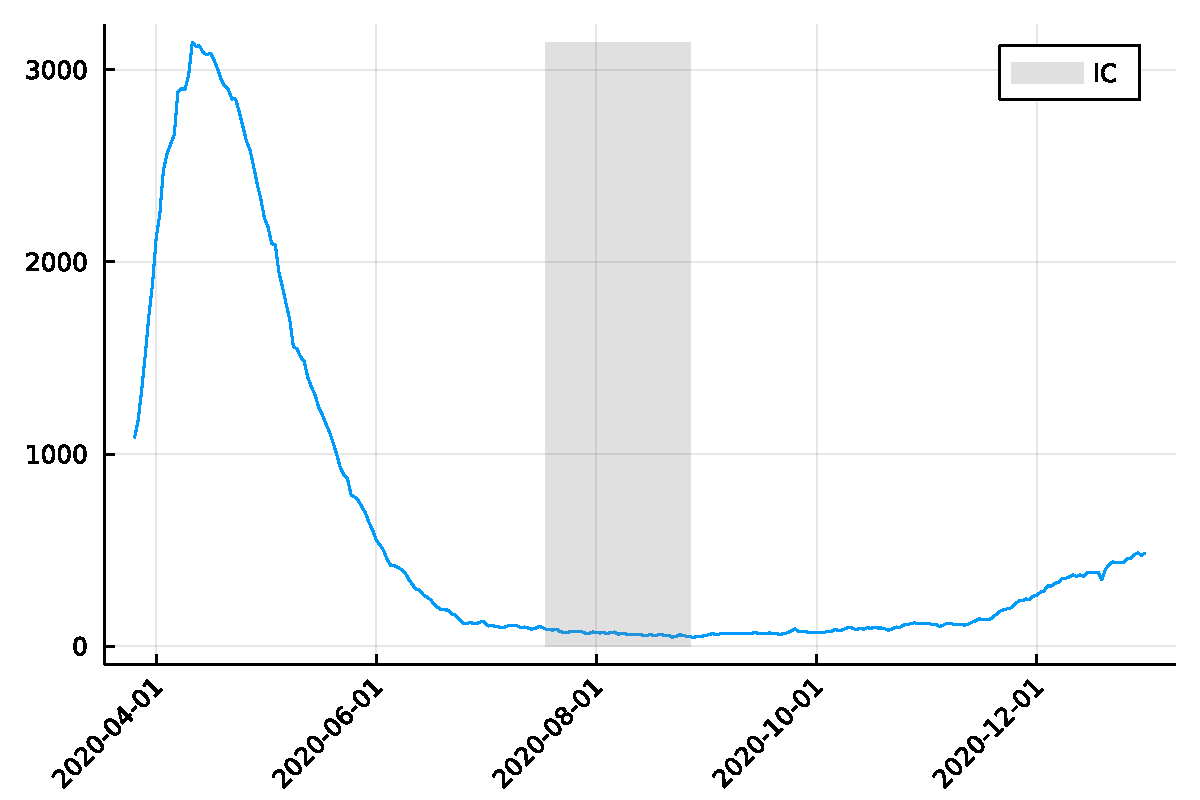
\includegraphics[width=\linewidth]{figures/admissionsICU_5_1.pdf}

We then isolate the IC and OC data. This code reproduces Figure ?? in the paper.


\begin{lstlisting}
(*@\HLJLn{y}@*) (*@\HLJLoB{=}@*) (*@\HLJLn{y2020}@*)(*@\HLJLp{[[}@*)(*@\HLJLn{ic{\_}2020}@*)(*@\HLJLp{;}@*) (*@\HLJLn{oc{\_}2020}@*)(*@\HLJLp{]]}@*)
(*@\HLJLn{days}@*) (*@\HLJLoB{=}@*) (*@\HLJLn{days2020}@*)(*@\HLJLp{[[}@*)(*@\HLJLn{ic{\_}2020}@*)(*@\HLJLp{;}@*) (*@\HLJLn{oc{\_}2020}@*)(*@\HLJLp{]]}@*)

(*@\HLJLn{ic{\_}idx}@*) (*@\HLJLoB{=}@*) (*@\HLJLni{1}@*)(*@\HLJLoB{:}@*)(*@\HLJLn{n{\_}ic}@*)
(*@\HLJLn{oc{\_}idx}@*) (*@\HLJLoB{=}@*) (*@\HLJLp{(}@*)(*@\HLJLn{n{\_}ic}@*)(*@\HLJLoB{+}@*)(*@\HLJLni{1}@*)(*@\HLJLp{)}@*)(*@\HLJLoB{:}@*)(*@\HLJLp{(}@*)(*@\HLJLn{n{\_}ic}@*)(*@\HLJLoB{+}@*)(*@\HLJLn{n{\_}oc}@*)(*@\HLJLp{)}@*)
(*@\HLJLn{yIC}@*) (*@\HLJLoB{=}@*) (*@\HLJLn{y}@*)(*@\HLJLp{[}@*)(*@\HLJLn{ic{\_}idx}@*)(*@\HLJLp{]}@*)
(*@\HLJLn{daysIC}@*) (*@\HLJLoB{=}@*) (*@\HLJLn{days}@*)(*@\HLJLp{[}@*)(*@\HLJLn{ic{\_}idx}@*)(*@\HLJLp{]}@*)
(*@\HLJLn{yOC}@*) (*@\HLJLoB{=}@*) (*@\HLJLn{y}@*)(*@\HLJLp{[}@*)(*@\HLJLn{oc{\_}idx}@*)(*@\HLJLp{]}@*)
(*@\HLJLn{daysOC}@*) (*@\HLJLoB{=}@*) (*@\HLJLn{days}@*)(*@\HLJLp{[}@*)(*@\HLJLn{oc{\_}idx}@*)(*@\HLJLp{]}@*)

(*@\HLJLnf{println}@*)(*@\HLJLp{(}@*)(*@\HLJLs{"{}In-control}@*) (*@\HLJLs{data:}@*) (*@\HLJLs{"{}}@*)(*@\HLJLp{,}@*) (*@\HLJLn{daysIC}@*)(*@\HLJLp{[[}@*)(*@\HLJLni{1}@*)(*@\HLJLp{,}@*) (*@\HLJLk{end}@*)(*@\HLJLp{]])}@*)
(*@\HLJLn{pl}@*) (*@\HLJLoB{=}@*) (*@\HLJLnf{plot}@*)(*@\HLJLp{(}@*)(*@\HLJLn{days}@*)(*@\HLJLp{,}@*) (*@\HLJLn{y}@*)(*@\HLJLp{,}@*) (*@\HLJLn{label}@*)(*@\HLJLoB{=}@*)(*@\HLJLs{"{}"{}}@*)(*@\HLJLp{,}@*) (*@\HLJLn{dpi}@*)(*@\HLJLoB{=}@*)(*@\HLJLni{400}@*)(*@\HLJLp{,}@*) (*@\HLJLn{xrotation}@*)(*@\HLJLoB{=}@*)(*@\HLJLni{45}@*)(*@\HLJLp{,}@*) (*@\HLJLn{bottom{\_}margin}@*)(*@\HLJLoB{=}@*)(*@\HLJLni{3}@*)(*@\HLJLn{mm}@*)(*@\HLJLp{)}@*)
(*@\HLJLnf{plot!}@*)(*@\HLJLp{(}@*)(*@\HLJLn{pl}@*)(*@\HLJLp{,}@*) (*@\HLJLn{days}@*)(*@\HLJLp{[}@*)(*@\HLJLni{1}@*)(*@\HLJLoB{:}@*)(*@\HLJLn{n{\_}ic}@*)(*@\HLJLp{],}@*) (*@\HLJLnf{fill}@*)(*@\HLJLp{(}@*)(*@\HLJLni{0}@*)(*@\HLJLp{,}@*) (*@\HLJLn{n{\_}ic}@*)(*@\HLJLp{),}@*) (*@\HLJLn{fillrange}@*)(*@\HLJLoB{=}@*)(*@\HLJLnf{fill}@*)(*@\HLJLp{(}@*)(*@\HLJLnf{maximum}@*)(*@\HLJLp{(}@*)(*@\HLJLn{y}@*)(*@\HLJLp{),}@*) (*@\HLJLn{n{\_}ic}@*)(*@\HLJLp{),}@*) (*@\HLJLn{color}@*)(*@\HLJLoB{=:}@*)(*@\HLJLn{gray}@*)(*@\HLJLp{,}@*) (*@\HLJLn{fillcolor}@*) (*@\HLJLoB{=}@*) (*@\HLJLs{"{}gray"{}}@*)(*@\HLJLp{,}@*) (*@\HLJLn{fillalpha}@*)(*@\HLJLoB{=}@*)(*@\HLJLnfB{0.25}@*)(*@\HLJLp{,}@*) (*@\HLJLn{alpha}@*)(*@\HLJLoB{=}@*)(*@\HLJLnfB{0.0}@*)(*@\HLJLp{,}@*) (*@\HLJLn{label}@*)(*@\HLJLoB{=}@*)(*@\HLJLs{"{}IC"{}}@*)(*@\HLJLp{,}@*) (*@\HLJLn{legend}@*)(*@\HLJLoB{=:}@*)(*@\HLJLn{bottomright}@*)(*@\HLJLp{)}@*)
(*@\HLJLn{\ensuremath{\tau}}@*) (*@\HLJLoB{=}@*) (*@\HLJLn{n{\_}ic}@*) (*@\HLJLoB{+}@*) (*@\HLJLni{29}@*)
(*@\HLJLnf{vline!}@*)(*@\HLJLp{([}@*)(*@\HLJLn{days}@*)(*@\HLJLp{[}@*)(*@\HLJLn{\ensuremath{\tau}}@*)(*@\HLJLp{]],}@*) (*@\HLJLn{color}@*)(*@\HLJLoB{=:}@*)(*@\HLJLn{gray}@*)(*@\HLJLp{,}@*) (*@\HLJLn{linestyle}@*)(*@\HLJLoB{=:}@*)(*@\HLJLn{dot}@*)(*@\HLJLp{,}@*) (*@\HLJLn{linewidth}@*)(*@\HLJLoB{=}@*)(*@\HLJLni{2}@*)(*@\HLJLp{,}@*)  (*@\HLJLn{label}@*)(*@\HLJLoB{=}@*)(*@\HLJLs{"{}"{}}@*)(*@\HLJLp{,}@*) (*@\HLJLn{markersize}@*)(*@\HLJLoB{=}@*)(*@\HLJLnfB{2.5}@*)(*@\HLJLp{)}@*)
(*@\HLJLnf{display}@*)(*@\HLJLp{(}@*)(*@\HLJLn{pl}@*)(*@\HLJLp{)}@*)

(*@\HLJLnf{println}@*)(*@\HLJLp{(}@*)(*@\HLJLs{"{}Possible}@*) (*@\HLJLs{change-point}@*) (*@\HLJLs{location:}@*) (*@\HLJLs{"{}}@*)(*@\HLJLp{,}@*) (*@\HLJLn{days}@*)(*@\HLJLp{[}@*)(*@\HLJLn{\ensuremath{\tau}}@*)(*@\HLJLp{])}@*)
\end{lstlisting}

\begin{lstlisting}
In-control data: [Dates.Date((*@{"{}}@*)2020-07-18(*@{"{}}@*)), Dates.Date((*@{"{}}@*)2020-08-27(*@{"{}}@*))]
Possible change-point location: 2020-09-25
\end{lstlisting}

\includegraphics[width=\linewidth]{figures/admissionsICU_6_1.pdf}

We can calculate the initial estimate $\hat{\theta}$ and set the desired nominal IC ARL of 500 alongside the GICP probability $\beta = 0.05$.


\begin{lstlisting}
(*@\HLJLn{Arl0}@*) (*@\HLJLoB{=}@*) (*@\HLJLni{500}@*)
(*@\HLJLn{beta}@*) (*@\HLJLoB{=}@*) (*@\HLJLnfB{0.05}@*)
(*@\HLJLn{thetaHat}@*) (*@\HLJLoB{=}@*) (*@\HLJLnf{mean}@*)(*@\HLJLp{(}@*)(*@\HLJLn{yIC}@*)(*@\HLJLp{)}@*)
(*@\HLJLnf{println}@*)(*@\HLJLp{(}@*)(*@\HLJLn{thetaHat}@*)(*@\HLJLp{)}@*)
\end{lstlisting}

\begin{lstlisting}
66.41463414634147
\end{lstlisting}


Next, we define a function that implements the control chart procedures using the various update mechanisms (AE, FE, CLM) that are defined in the source code.


\begin{lstlisting}
(*@\HLJLk{function}@*) (*@\HLJLnf{applyChart}@*)(*@\HLJLp{(}@*)(*@\HLJLn{ch}@*)(*@\HLJLp{,}@*) (*@\HLJLn{um}@*)(*@\HLJLp{,}@*) (*@\HLJLn{thetaHat}@*)(*@\HLJLp{,}@*) (*@\HLJLn{m}@*)(*@\HLJLp{,}@*) (*@\HLJLn{yprosp}@*)(*@\HLJLp{;}@*) (*@\HLJLn{seed}@*) (*@\HLJLoB{=}@*) (*@\HLJLni{123}@*)(*@\HLJLp{)}@*)
    (*@\HLJLcs{{\#}}@*) (*@\HLJLcs{Random.seed!(seed)}@*)
    (*@\HLJLn{maxrl{\_}i}@*) (*@\HLJLoB{=}@*) (*@\HLJLnf{length}@*)(*@\HLJLp{(}@*)(*@\HLJLn{yprosp}@*)(*@\HLJLp{)}@*)
    (*@\HLJLn{thetaHatVec}@*) (*@\HLJLoB{=}@*) (*@\HLJLnf{zeros}@*)(*@\HLJLp{(}@*)(*@\HLJLn{maxrl{\_}i}@*)(*@\HLJLp{)}@*)
    (*@\HLJLn{thetaHatVec}@*)(*@\HLJLp{[}@*)(*@\HLJLni{1}@*)(*@\HLJLp{]}@*) (*@\HLJLoB{=}@*) (*@\HLJLn{thetaHat}@*)
    (*@\HLJLn{di}@*) (*@\HLJLoB{=}@*) (*@\HLJLni{1}@*)
    (*@\HLJLn{diVec}@*) (*@\HLJLoB{=}@*) (*@\HLJLnf{Array}@*)(*@\HLJLp{{\{}}@*)(*@\HLJLn{Int}@*)(*@\HLJLp{{\}}(}@*)(*@\HLJLn{undef}@*)(*@\HLJLp{,}@*) (*@\HLJLn{maxrl{\_}i}@*)(*@\HLJLp{)}@*)
    (*@\HLJLn{diVec}@*)(*@\HLJLp{[}@*)(*@\HLJLni{1}@*)(*@\HLJLp{]}@*) (*@\HLJLoB{=}@*) (*@\HLJLn{di}@*)
    (*@\HLJLn{thetaHatCaut}@*) (*@\HLJLoB{=}@*) (*@\HLJLn{thetaHat}@*)
    (*@\HLJLn{thetaHatCautVec}@*) (*@\HLJLoB{=}@*) (*@\HLJLnf{zeros}@*)(*@\HLJLp{(}@*)(*@\HLJLn{maxrl{\_}i}@*)(*@\HLJLp{)}@*)
    (*@\HLJLn{thetaHatCautVec}@*)(*@\HLJLp{[}@*)(*@\HLJLni{1}@*)(*@\HLJLp{]}@*) (*@\HLJLoB{=}@*) (*@\HLJLn{thetaHatCaut}@*)

    (*@\HLJLn{t{\_}alarm}@*) (*@\HLJLoB{=}@*) (*@\HLJLnf{zeros}@*)(*@\HLJLp{(}@*)(*@\HLJLni{0}@*)(*@\HLJLp{)}@*)

    (*@\HLJLn{valueVec}@*) (*@\HLJLoB{=}@*) (*@\HLJLnf{zeros}@*)(*@\HLJLp{(}@*)(*@\HLJLn{maxrl{\_}i}@*)(*@\HLJLp{)}@*)
    (*@\HLJLn{valueVec}@*)(*@\HLJLp{[}@*)(*@\HLJLni{1}@*)(*@\HLJLp{]}@*) (*@\HLJLoB{=}@*) (*@\HLJLnf{get{\_}value}@*)(*@\HLJLp{(}@*)(*@\HLJLn{ch}@*)(*@\HLJLp{)}@*)
    (*@\HLJLn{i}@*) (*@\HLJLoB{=}@*) (*@\HLJLni{1}@*)
    (*@\HLJLk{while}@*) (*@\HLJLn{i}@*) (*@\HLJLoB{<}@*) (*@\HLJLn{maxrl{\_}i}@*)
        (*@\HLJLn{thetaHatCaut}@*) (*@\HLJLoB{=}@*) (*@\HLJLn{thetaHatVec}@*)(*@\HLJLp{[}@*)(*@\HLJLn{i}@*) (*@\HLJLoB{-}@*) (*@\HLJLn{di}@*) (*@\HLJLoB{+}@*) (*@\HLJLni{1}@*)(*@\HLJLp{]}@*)
        (*@\HLJLn{y}@*) (*@\HLJLoB{=}@*) (*@\HLJLn{yprosp}@*)(*@\HLJLp{[}@*)(*@\HLJLn{i}@*)(*@\HLJLp{]}@*)
        (*@\HLJLn{ch}@*) (*@\HLJLoB{=}@*) (*@\HLJLnf{update{\_}series}@*)(*@\HLJLp{(}@*)(*@\HLJLn{ch}@*)(*@\HLJLp{,}@*) (*@\HLJLnf{chart{\_}statistic}@*)(*@\HLJLp{(}@*)(*@\HLJLn{y}@*)(*@\HLJLp{,}@*) (*@\HLJLn{thetaHatCaut}@*)(*@\HLJLp{))}@*)
        (*@\HLJLn{thetaHat}@*) (*@\HLJLoB{=}@*) (*@\HLJLnf{update{\_}parameter}@*)(*@\HLJLp{(}@*)(*@\HLJLn{thetaHat}@*)(*@\HLJLp{,}@*) (*@\HLJLn{y}@*)(*@\HLJLp{,}@*) (*@\HLJLn{i}@*) (*@\HLJLoB{+}@*) (*@\HLJLn{m}@*)(*@\HLJLp{)}@*)
        (*@\HLJLn{i}@*) (*@\HLJLoB{+=}@*) (*@\HLJLni{1}@*)
        (*@\HLJLn{valueVec}@*)(*@\HLJLp{[}@*)(*@\HLJLn{i}@*)(*@\HLJLp{]}@*) (*@\HLJLoB{=}@*) (*@\HLJLnf{get{\_}value}@*)(*@\HLJLp{(}@*)(*@\HLJLn{ch}@*)(*@\HLJLp{)}@*)
        (*@\HLJLn{thetaHatVec}@*)(*@\HLJLp{[}@*)(*@\HLJLn{i}@*)(*@\HLJLp{]}@*) (*@\HLJLoB{=}@*) (*@\HLJLn{thetaHat}@*)
        (*@\HLJLk{if}@*) (*@\HLJLnf{check{\_}update}@*)(*@\HLJLp{(}@*)(*@\HLJLn{ch}@*)(*@\HLJLp{,}@*) (*@\HLJLn{um}@*)(*@\HLJLp{)}@*)
            (*@\HLJLn{di}@*) (*@\HLJLoB{=}@*) (*@\HLJLni{1}@*)
        (*@\HLJLk{else}@*)
            (*@\HLJLn{di}@*) (*@\HLJLoB{+=}@*) (*@\HLJLni{1}@*)
        (*@\HLJLk{end}@*)
        (*@\HLJLn{diVec}@*)(*@\HLJLp{[}@*)(*@\HLJLn{i}@*)(*@\HLJLp{]}@*) (*@\HLJLoB{=}@*) (*@\HLJLn{di}@*)
        (*@\HLJLn{thetaHatCautVec}@*)(*@\HLJLp{[}@*)(*@\HLJLn{i}@*)(*@\HLJLp{]}@*) (*@\HLJLoB{=}@*) (*@\HLJLn{thetaHatCaut}@*)
        (*@\HLJLk{if}@*) (*@\HLJLnf{check{\_}OC}@*)(*@\HLJLp{(}@*)(*@\HLJLn{ch}@*)(*@\HLJLp{)}@*)
            (*@\HLJLnf{push!}@*)(*@\HLJLp{(}@*)(*@\HLJLn{t{\_}alarm}@*)(*@\HLJLp{,}@*) (*@\HLJLn{i}@*)(*@\HLJLp{)}@*)
        (*@\HLJLk{end}@*)
    (*@\HLJLk{end}@*)

    (*@\HLJLk{return}@*) (*@\HLJLp{(}@*)(*@\HLJLn{t{\_}alarm}@*) (*@\HLJLoB{=}@*) (*@\HLJLn{t{\_}alarm}@*)(*@\HLJLp{,}@*) (*@\HLJLn{dat}@*) (*@\HLJLoB{=}@*) (*@\HLJLn{yprosp}@*)(*@\HLJLp{,}@*) (*@\HLJLn{chart{\_}values}@*) (*@\HLJLoB{=}@*) (*@\HLJLn{valueVec}@*)(*@\HLJLp{,}@*) (*@\HLJLn{limit{\_}alarm}@*) (*@\HLJLoB{=}@*) (*@\HLJLnf{get{\_}limits}@*)(*@\HLJLp{(}@*)(*@\HLJLn{ch}@*)(*@\HLJLp{),}@*) (*@\HLJLn{limit{\_}cautious}@*) (*@\HLJLoB{=}@*) (*@\HLJLnf{get{\_}warning{\_}limit}@*)(*@\HLJLp{(}@*)(*@\HLJLn{um}@*)(*@\HLJLp{),}@*) (*@\HLJLn{parameter{\_}updates}@*) (*@\HLJLoB{=}@*) (*@\HLJLn{thetaHatCautVec}@*)(*@\HLJLp{,}@*) (*@\HLJLn{di}@*) (*@\HLJLoB{=}@*) (*@\HLJLn{diVec}@*)(*@\HLJLp{)}@*)
(*@\HLJLk{end}@*)
\end{lstlisting}

\begin{lstlisting}
applyChart (generic function with 1 method)
\end{lstlisting}


The function arguments are:

\begin{itemize}
\item \texttt{ch}: an \texttt{AbstractSeries} object, as defined in the \texttt{StatisticalProcessControl} package that is shipped with the source code.


\item \texttt{um}: an \texttt{AbstractUpdate} object, as defined in the \texttt{StatisticalProcessControl} package that is shipped with the source code.


\item \texttt{thetaHat}: the estimate of the IC mean.


\item \texttt{m}: the initial sample size.


\item \texttt{yprosp}: data onto which the control chart must be applied.


\item \texttt{seed}: eventual seed that is passed to the GICP optimization for reproducibility. 

\end{itemize}
When the above function is called sequence of count data, the returned values are

\begin{itemize}
\item \texttt{t\_alarm}: the time of the first alarm.


\item \texttt{dat}: the data onto which the control chart was applied.


\item \texttt{chart\_values}: the vector of values of the control chart.


\item \texttt{limit\_alarm}: the control chart limit.


\item \texttt{limit\_cautious}: if the control chart has a warning region, this contains the value.


\item \texttt{parameter\_updates}: the sequence of parameter values.


\item \texttt{di}: the sequence of $d_t$'s.

\end{itemize}
Furthermore, we define a function that applies the control chart to a prospective monitoring data after having corrected the control limit to satisfy the GICP condition.


\begin{lstlisting}
(*@\HLJLk{function}@*) (*@\HLJLnf{applyChartGICP}@*)(*@\HLJLp{(}@*)(*@\HLJLn{ch}@*)(*@\HLJLp{,}@*) (*@\HLJLn{um}@*)(*@\HLJLp{,}@*) (*@\HLJLn{yinit}@*)(*@\HLJLp{,}@*) (*@\HLJLn{yprosp}@*)(*@\HLJLp{,}@*) (*@\HLJLn{thetaHat}@*)(*@\HLJLp{,}@*) (*@\HLJLn{Arl0}@*)(*@\HLJLp{;}@*) (*@\HLJLn{beta}@*)(*@\HLJLoB{::}@*)(*@\HLJLnf{Union}@*)(*@\HLJLp{{\{}}@*)(*@\HLJLn{Bool}@*)(*@\HLJLp{,}@*) (*@\HLJLn{Float64}@*)(*@\HLJLp{{\}}}@*) (*@\HLJLoB{=}@*) (*@\HLJLnfB{0.2}@*)(*@\HLJLp{,}@*) (*@\HLJLn{maxrl}@*)(*@\HLJLoB{=}@*)(*@\HLJLnfB{1e04}@*)(*@\HLJLp{,}@*) (*@\HLJLn{verbose}@*)(*@\HLJLoB{=}@*)(*@\HLJLkc{true}@*)(*@\HLJLp{,}@*) (*@\HLJLn{seed}@*)(*@\HLJLoB{=}@*)(*@\HLJLnf{Int}@*)(*@\HLJLp{(}@*)(*@\HLJLnf{rand}@*)(*@\HLJLp{(}@*)(*@\HLJLni{1}@*)(*@\HLJLoB{:}@*)(*@\HLJLnfB{1e06}@*)(*@\HLJLp{)))}@*)
    (*@\HLJLn{m}@*) (*@\HLJLoB{=}@*) (*@\HLJLnf{length}@*)(*@\HLJLp{(}@*)(*@\HLJLn{yinit}@*)(*@\HLJLp{)}@*)
    (*@\HLJLk{if}@*) (*@\HLJLnf{isa}@*)(*@\HLJLp{(}@*)(*@\HLJLn{um}@*)(*@\HLJLp{,}@*) (*@\HLJLn{CautiousLearning}@*)(*@\HLJLp{)}@*)
        (*@\HLJLn{Ats0}@*) (*@\HLJLoB{=}@*) (*@\HLJLnf{get{\_}ATS}@*)(*@\HLJLp{(}@*)(*@\HLJLn{um}@*)(*@\HLJLp{)}@*)
        (*@\HLJLk{if}@*) (*@\HLJLn{Ats0}@*) (*@\HLJLoB{!=}@*) (*@\HLJLni{0}@*)
            (*@\HLJLcs{{\#}}@*) (*@\HLJLcs{Calculate}@*) (*@\HLJLcs{limit}@*) (*@\HLJLcs{if}@*) (*@\HLJLcs{Ats0}@*) (*@\HLJLcs{!=}@*) (*@\HLJLcs{0,}@*) (*@\HLJLcs{otherwise}@*) (*@\HLJLcs{use}@*) (*@\HLJLcs{zero-restarting}@*) (*@\HLJLcs{chart}@*)
            (*@\HLJLk{if}@*) (*@\HLJLn{verbose}@*) (*@\HLJLnf{println}@*)(*@\HLJLp{(}@*)(*@\HLJLs{"{}Calculating}@*) (*@\HLJLs{limits}@*) (*@\HLJLs{for}@*) (*@\HLJLs{target}@*) (*@\HLJLs{ATS..."{}}@*)(*@\HLJLp{)}@*) (*@\HLJLk{end}@*)
            (*@\HLJLn{sa{\_}ats}@*) (*@\HLJLoB{=}@*) (*@\HLJLnf{saControlLimits}@*)(*@\HLJLp{(}@*)(*@\HLJLn{ch}@*)(*@\HLJLp{,}@*) (*@\HLJLnf{AdaptiveEstimator}@*)(*@\HLJLp{(),}@*) (*@\HLJLn{runSimulation}@*)(*@\HLJLp{,}@*) (*@\HLJLn{Ats0}@*)(*@\HLJLp{,}@*) (*@\HLJLn{thetaHat}@*)(*@\HLJLp{,}@*) (*@\HLJLnf{Poisson}@*)(*@\HLJLp{(}@*)(*@\HLJLn{thetaHat}@*)(*@\HLJLp{),}@*)
                                    (*@\HLJLn{m}@*)(*@\HLJLp{,}@*) (*@\HLJLn{verbose}@*)(*@\HLJLoB{=}@*)(*@\HLJLkc{false}@*)(*@\HLJLp{,}@*) (*@\HLJLn{Amin}@*)(*@\HLJLoB{=}@*)(*@\HLJLnfB{0.1}@*)(*@\HLJLp{,}@*) (*@\HLJLn{maxiter}@*)(*@\HLJLoB{=}@*)(*@\HLJLnfB{1e05}@*)(*@\HLJLp{,}@*)
                                    (*@\HLJLn{gamma}@*)(*@\HLJLoB{=}@*)(*@\HLJLnfB{0.015}@*)(*@\HLJLp{,}@*) (*@\HLJLn{adjusted}@*)(*@\HLJLoB{=}@*)(*@\HLJLkc{true}@*)(*@\HLJLp{,}@*) (*@\HLJLn{seed}@*)(*@\HLJLoB{=}@*)(*@\HLJLn{seed}@*)(*@\HLJLp{)}@*)
            (*@\HLJLn{um}@*) (*@\HLJLoB{=}@*) (*@\HLJLnf{CautiousLearning}@*)(*@\HLJLp{(}@*)(*@\HLJLn{L}@*) (*@\HLJLoB{=}@*) (*@\HLJLn{sa{\_}ats}@*)(*@\HLJLp{[}@*)(*@\HLJLsc{:h}@*)(*@\HLJLp{],}@*) (*@\HLJLn{ATS}@*) (*@\HLJLoB{=}@*) (*@\HLJLn{Ats0}@*)(*@\HLJLp{)}@*)
        (*@\HLJLk{else}@*)
            (*@\HLJLk{if}@*) (*@\HLJLn{verbose}@*) (*@\HLJLnf{println}@*)(*@\HLJLp{(}@*)(*@\HLJLs{"{}ATS}@*) (*@\HLJLs{=}@*) (*@\HLJLs{0,}@*) (*@\HLJLs{skipping}@*) (*@\HLJLs{limit}@*) (*@\HLJLs{calculation."{}}@*)(*@\HLJLp{)}@*) (*@\HLJLk{end}@*)
        (*@\HLJLk{end}@*)
        (*@\HLJLcs{{\#}}@*) (*@\HLJLcs{Estimate}@*) (*@\HLJLcs{cautious}@*) (*@\HLJLcs{learning}@*) (*@\HLJLcs{limit}@*)
    (*@\HLJLk{end}@*)

    (*@\HLJLk{if}@*) (*@\HLJLn{beta}@*) (*@\HLJLoB{==}@*) (*@\HLJLkc{false}@*)
        (*@\HLJLn{chart}@*) (*@\HLJLoB{=}@*) (*@\HLJLnf{deepcopy}@*)(*@\HLJLp{(}@*)(*@\HLJLn{ch}@*)(*@\HLJLp{)}@*)
    (*@\HLJLk{else}@*)
        (*@\HLJLn{chart}@*) (*@\HLJLoB{=}@*) (*@\HLJLnf{adjust{\_}chart{\_}gicp}@*)(*@\HLJLp{(}@*)(*@\HLJLn{ch}@*)(*@\HLJLp{,}@*) (*@\HLJLn{um}@*)(*@\HLJLp{,}@*) (*@\HLJLn{yinit}@*)(*@\HLJLp{,}@*) (*@\HLJLn{thetaHat}@*)(*@\HLJLp{,}@*) (*@\HLJLn{runSimulation}@*)(*@\HLJLp{,}@*) (*@\HLJLn{m}@*)(*@\HLJLp{,}@*) (*@\HLJLn{Arl0}@*)(*@\HLJLp{,}@*) (*@\HLJLn{beta}@*)(*@\HLJLoB{=}@*)(*@\HLJLn{beta}@*)(*@\HLJLp{,}@*) (*@\HLJLn{verbose}@*)(*@\HLJLoB{=}@*)(*@\HLJLn{verbose}@*)(*@\HLJLp{)}@*)
    (*@\HLJLk{end}@*)

    (*@\HLJLk{return}@*) (*@\HLJLnf{applyChart}@*)(*@\HLJLp{(}@*)(*@\HLJLn{chart}@*)(*@\HLJLp{,}@*) (*@\HLJLn{um}@*)(*@\HLJLp{,}@*) (*@\HLJLn{thetaHat}@*)(*@\HLJLp{,}@*) (*@\HLJLn{m}@*)(*@\HLJLp{,}@*) (*@\HLJLn{yprosp}@*)(*@\HLJLp{)}@*)
(*@\HLJLk{end}@*)
\end{lstlisting}

\begin{lstlisting}
applyChartGICP (generic function with 1 method)
\end{lstlisting}


The GICP control limit correction uses the \texttt{adjust\_chart\_gicp} function defined in the source code, which implements the control limit computation described in Subsection ??.

We finally apply the control charts using the methods and obtain the results.  This code reproduces Figure ?? and Table ??.


\begin{lstlisting}
(*@\HLJLn{Random}@*)(*@\HLJLoB{.}@*)(*@\HLJLnf{seed!}@*)(*@\HLJLp{(}@*)(*@\HLJLni{2022}@*)(*@\HLJLoB{-}@*)(*@\HLJLni{08}@*)(*@\HLJLoB{-}@*)(*@\HLJLni{18}@*)(*@\HLJLp{)}@*)
(*@\HLJLn{D}@*) (*@\HLJLoB{=}@*) (*@\HLJLn{Poisson}@*)
(*@\HLJLn{fname}@*) (*@\HLJLoB{=}@*) (*@\HLJLnf{plotsdir}@*)(*@\HLJLp{(}@*)(*@\HLJLn{fold}@*)(*@\HLJLp{,}@*) (*@\HLJLs{"{}alarms.jld2"{}}@*)(*@\HLJLp{)}@*)

(*@\HLJLn{umVec}@*) (*@\HLJLoB{=}@*) (*@\HLJLp{[}@*)(*@\HLJLnf{CautiousLearning}@*)(*@\HLJLp{(}@*)(*@\HLJLn{ATS}@*)(*@\HLJLoB{=}@*)(*@\HLJLni{0}@*)(*@\HLJLp{),}@*) (*@\HLJLnf{FixedParameter}@*)(*@\HLJLp{(),}@*) (*@\HLJLnf{AdaptiveEstimator}@*)(*@\HLJLp{()]}@*)
(*@\HLJLn{nms}@*) (*@\HLJLoB{=}@*) (*@\HLJLp{[}@*)(*@\HLJLs{"{}CLM"{}}@*)(*@\HLJLp{,}@*) (*@\HLJLs{"{}FE"{}}@*)(*@\HLJLp{,}@*) (*@\HLJLs{"{}AE"{}}@*)(*@\HLJLp{]}@*)
(*@\HLJLn{perf}@*) (*@\HLJLoB{=}@*) (*@\HLJLp{[]}@*)
(*@\HLJLn{L}@*) (*@\HLJLoB{=}@*) (*@\HLJLp{[]}@*)
(*@\HLJLk{for}@*) (*@\HLJLn{i}@*) (*@\HLJLkp{in}@*) (*@\HLJLnf{eachindex}@*)(*@\HLJLp{(}@*)(*@\HLJLn{umVec}@*)(*@\HLJLp{)}@*)
    (*@\HLJLn{ch}@*) (*@\HLJLoB{=}@*) (*@\HLJLnf{signedEWMA}@*)(*@\HLJLp{(}@*)(*@\HLJLn{l}@*)(*@\HLJLoB{=}@*)(*@\HLJLnfB{0.2}@*)(*@\HLJLp{,}@*) (*@\HLJLn{L}@*) (*@\HLJLoB{=}@*) (*@\HLJLnfB{1.0}@*)(*@\HLJLp{)}@*)
    (*@\HLJLn{um}@*) (*@\HLJLoB{=}@*) (*@\HLJLn{umVec}@*)(*@\HLJLp{[}@*)(*@\HLJLn{i}@*)(*@\HLJLp{]}@*)
    (*@\HLJLn{res}@*) (*@\HLJLoB{=}@*) (*@\HLJLnf{applyChartGICP}@*)(*@\HLJLp{(}@*)(*@\HLJLn{ch}@*)(*@\HLJLp{,}@*) (*@\HLJLn{um}@*)(*@\HLJLp{,}@*) (*@\HLJLn{yIC}@*)(*@\HLJLp{,}@*) (*@\HLJLn{yOC}@*)(*@\HLJLp{,}@*) (*@\HLJLn{thetaHat}@*)(*@\HLJLp{,}@*) (*@\HLJLn{Arl0}@*)(*@\HLJLp{,}@*) (*@\HLJLn{beta}@*)(*@\HLJLoB{=}@*)(*@\HLJLn{beta}@*)(*@\HLJLp{)}@*)
    (*@\HLJLnf{append!}@*)(*@\HLJLp{(}@*)(*@\HLJLn{L}@*)(*@\HLJLp{,}@*) (*@\HLJLn{res}@*)(*@\HLJLp{[}@*)(*@\HLJLsc{:limit{\_}alarm}@*)(*@\HLJLp{])}@*)
    (*@\HLJLn{plotsave}@*) (*@\HLJLoB{=}@*) (*@\HLJLnf{plotsdir}@*)(*@\HLJLp{(}@*)(*@\HLJLn{fold}@*)(*@\HLJLp{,}@*) (*@\HLJLn{nms}@*)(*@\HLJLp{[}@*)(*@\HLJLn{i}@*)(*@\HLJLp{]}@*)(*@\HLJLoB{*}@*)(*@\HLJLs{"{}.png"{}}@*)(*@\HLJLp{)}@*)
    (*@\HLJLn{pl}@*) (*@\HLJLoB{=}@*) (*@\HLJLnf{plot}@*)(*@\HLJLp{(}@*)(*@\HLJLn{res}@*)(*@\HLJLoB{.}@*)(*@\HLJLn{chart{\_}values}@*)(*@\HLJLp{[}@*)(*@\HLJLni{1}@*)(*@\HLJLoB{:}@*)(*@\HLJLni{55}@*)(*@\HLJLp{],}@*) (*@\HLJLn{label}@*)(*@\HLJLoB{=}@*)(*@\HLJLso{L"{}C{\_}t"{}}@*)(*@\HLJLp{,}@*) (*@\HLJLn{legend}@*)(*@\HLJLoB{=:}@*)(*@\HLJLn{outerright}@*)(*@\HLJLp{,}@*) (*@\HLJLn{dpi}@*)(*@\HLJLoB{=}@*)(*@\HLJLni{400}@*)(*@\HLJLp{)}@*)
    (*@\HLJLnf{hline!}@*)(*@\HLJLp{([}@*)(*@\HLJLn{res}@*)(*@\HLJLoB{.}@*)(*@\HLJLn{limit{\_}alarm}@*)(*@\HLJLp{],}@*) (*@\HLJLn{style}@*)(*@\HLJLoB{=:}@*)(*@\HLJLn{dash}@*)(*@\HLJLp{,}@*) (*@\HLJLn{colour}@*)(*@\HLJLoB{=}@*)(*@\HLJLs{"{}red"{}}@*)(*@\HLJLp{,}@*) (*@\HLJLn{xlab}@*)(*@\HLJLoB{=}@*)(*@\HLJLso{L"{}t"{}}@*)(*@\HLJLp{,}@*) (*@\HLJLn{ylab}@*)(*@\HLJLoB{=}@*)(*@\HLJLso{L"{}C{\_}t"{}}@*)(*@\HLJLp{,}@*) (*@\HLJLn{label}@*)(*@\HLJLoB{=}@*)(*@\HLJLs{"{}"{}}@*)(*@\HLJLp{)}@*)
    (*@\HLJLn{tau}@*) (*@\HLJLoB{=}@*) (*@\HLJLnf{Int}@*)(*@\HLJLp{(}@*)(*@\HLJLnf{first}@*)(*@\HLJLp{(}@*)(*@\HLJLn{res}@*)(*@\HLJLoB{.}@*)(*@\HLJLn{t{\_}alarm}@*)(*@\HLJLp{))}@*)
    (*@\HLJLnf{scatter!}@*)(*@\HLJLp{([}@*)(*@\HLJLn{tau}@*)(*@\HLJLp{],}@*) (*@\HLJLp{[}@*)(*@\HLJLn{res}@*)(*@\HLJLoB{.}@*)(*@\HLJLn{chart{\_}values}@*)(*@\HLJLp{[}@*)(*@\HLJLn{tau}@*)(*@\HLJLp{]],}@*) (*@\HLJLn{colour}@*)(*@\HLJLoB{=}@*)(*@\HLJLs{"{}red"{}}@*)(*@\HLJLp{,}@*) (*@\HLJLn{label}@*)(*@\HLJLoB{=}@*)(*@\HLJLs{"{}"{}}@*)(*@\HLJLp{)}@*)
    (*@\HLJLnf{display}@*)(*@\HLJLp{(}@*)(*@\HLJLn{pl}@*)(*@\HLJLp{)}@*)
    (*@\HLJLnf{append!}@*)(*@\HLJLp{(}@*)(*@\HLJLn{perf}@*)(*@\HLJLp{,}@*) (*@\HLJLn{tau}@*)(*@\HLJLp{)}@*)
    (*@\HLJLnf{println}@*)(*@\HLJLp{(}@*)(*@\HLJLn{tau}@*)(*@\HLJLp{,}@*)(*@\HLJLs{"{}}@*)(*@\HLJLse{{\textbackslash}t}@*)(*@\HLJLs{"{}}@*)(*@\HLJLp{,}@*) (*@\HLJLn{daysOC}@*)(*@\HLJLp{[}@*)(*@\HLJLn{tau}@*)(*@\HLJLp{])}@*)
(*@\HLJLk{end}@*)

(*@\HLJLnd{@rput}@*) (*@\HLJLn{nms}@*)
(*@\HLJLnd{@rput}@*) (*@\HLJLn{perf}@*)
(*@\HLJLnd{@rput}@*) (*@\HLJLn{L}@*)

(*@\HLJLn{tab}@*) (*@\HLJLoB{=}@*) (*@\HLJLso{R"{}"{}"{}}@*)
(*@\HLJLso{library(knitr)}@*)
(*@\HLJLso{library(kableExtra)}@*)
(*@\HLJLso{df}@*) (*@\HLJLso{=}@*) (*@\HLJLso{cbind(nms,}@*) (*@\HLJLso{perf,}@*) (*@\HLJLso{L)}@*)
(*@\HLJLso{tex{\_}OC}@*) (*@\HLJLso{<-}@*) (*@\HLJLso{kable(df,}@*) (*@\HLJLso{format="{}latex"{},}@*) (*@\HLJLso{digits}@*) (*@\HLJLso{=}@*) (*@\HLJLso{2,}@*) (*@\HLJLso{row.names=FALSE,}@*) (*@\HLJLso{col.names=c("{}Estimator"{},}@*) (*@\HLJLso{"{}Alarm"{},}@*) (*@\HLJLso{"{}Limit"{}),}@*) (*@\HLJLso{escape=FALSE,}@*) (*@\HLJLso{align={\textquotesingle}c{\textquotesingle},}@*) (*@\HLJLso{linesep}@*) (*@\HLJLso{=}@*) (*@\HLJLso{"{}"{},}@*)
    (*@\HLJLso{caption}@*) (*@\HLJLso{=}@*) (*@\HLJLso{"{}Time}@*) (*@\HLJLso{to}@*) (*@\HLJLso{alarm}@*) (*@\HLJLso{of}@*) (*@\HLJLso{the}@*) (*@\HLJLso{one-sided}@*) (*@\HLJLso{EWMA}@*) (*@\HLJLso{control}@*) (*@\HLJLso{chart}@*) (*@\HLJLso{using}@*) (*@\HLJLso{the}@*) (*@\HLJLso{fixed}@*) (*@\HLJLso{(FE),}@*) (*@\HLJLso{adaptive}@*) (*@\HLJLso{(AE)}@*) (*@\HLJLso{and}@*) (*@\HLJLso{the}@*) (*@\HLJLso{proposed}@*) (*@\HLJLso{cautious}@*) (*@\HLJLso{learning}@*) (*@\HLJLso{(CLM)}@*) (*@\HLJLso{update}@*) (*@\HLJLso{rules."{},}@*) (*@\HLJLso{label="{}ICU}@*) (*@\HLJLso{OC}@*) (*@\HLJLso{alarm"{})}@*)
(*@\HLJLso{"{}"{}"{}}@*) (*@\HLJLoB{|>}@*) (*@\HLJLn{rcopy}@*)

(*@\HLJLnf{println}@*)(*@\HLJLp{(}@*)(*@\HLJLn{tab}@*)(*@\HLJLp{)}@*)
\end{lstlisting}

\begin{lstlisting}
ATS = 0, skipping limit calculation.
Calculating GICP for extremum 1/1...
GICP done.
30	2020-09-26
Calculating GICP for extremum 1/1...
GICP done.
41	2020-10-07
Calculating GICP for extremum 1/1...
GICP done.
31	2020-09-27
\end{lstlisting}

\begin{table}

\caption{\label{tab:ICU OC alarm}Time to alarm of the one-sided EWMA control chart using the fixed (FE), adaptive (AE) and the proposed cautious learning (CLM) update rules.}
\centering
\begin{tabular}[t]{c|c|c}
\hline
Estimator & Alarm & Limit\\
\hline
CLM & 30 & 1.05469060798468\\
FE & 41 & 1.2147825075143\\
AE & 31 & 1.02214273823991\\
\hline
\end{tabular}
\end{table}

\includegraphics[width=\linewidth]{figures/admissionsICU_10_1.pdf}
\includegraphics[width=\linewidth]{figures/admissionsICU_10_2.pdf}
\includegraphics[width=\linewidth]{figures/admissionsICU_10_3.pdf}


\end{document}
